\chapter*{Cronograma}

A seguir temos o cronograma das atividades que foram e que serão desenvolvidas no decorrer do curso de pós graduação.
    
\begin{figure}[ht]
	\centering
	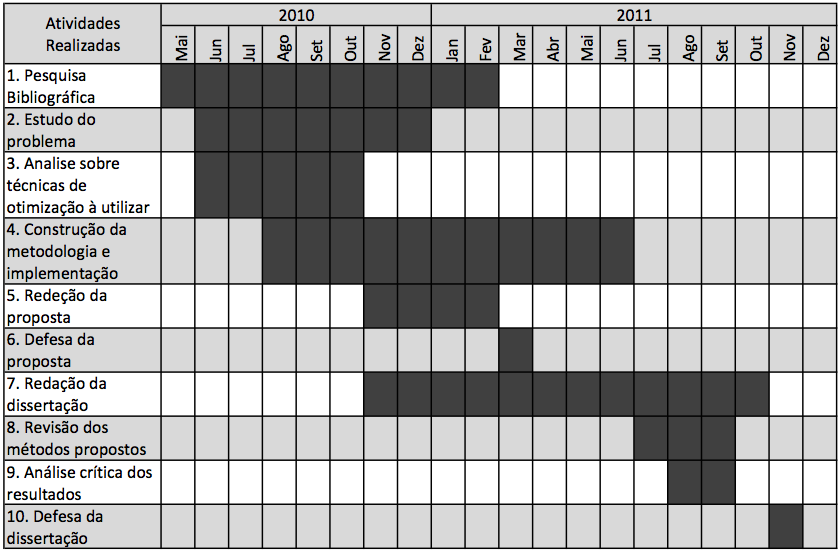
\includegraphics[scale=0.48]{./img/cronograma}
	%\caption{Heurística de construção aleatória de uma solução inicial}
	\label{cronograma}
 \end{figure}
    
Inicialmente foi feito um levantamento bibliográfico sobre o PCTA e outros que são correlatos ou similares a ele, também foi pesquisado sobre metaheurísticas que tiveram bons resultados com esses tipos de problemas. Em seguida foi estudado a possibilidade de integração da metaheurística escolhida com alguma modelagem matemática eficiente. Após isso foi elaborado e implementado o método proposto.

Fica faltando ainda a finalização dessa implementação e a revisão do método proposto, bem como a análise crítica dos resultados. Após essa parte a redação da dissertação para posterior defesa da mesma. O mês de dezembro fica vago para o caso de ocorrer algum imprevisto no decorrer da execução do cronograma.
